\subsection{Диаграмма Ганта} \label{gant}

Для иллюстрации последовательности проводимых работ приведем диаграмму Ганта данного проекта, на которой по оси $X$ изображены календарные дни от начала до конца проекта, а по оси $Y$ – выполняемые этапы работ.
Диаграмма Ганта приведена на рисунке \ref{img:gant_diagram}. Занятость исполнителей приведена в таблице \ref{table:workers_dates}.

\begin{figure} [h] 
  \center
  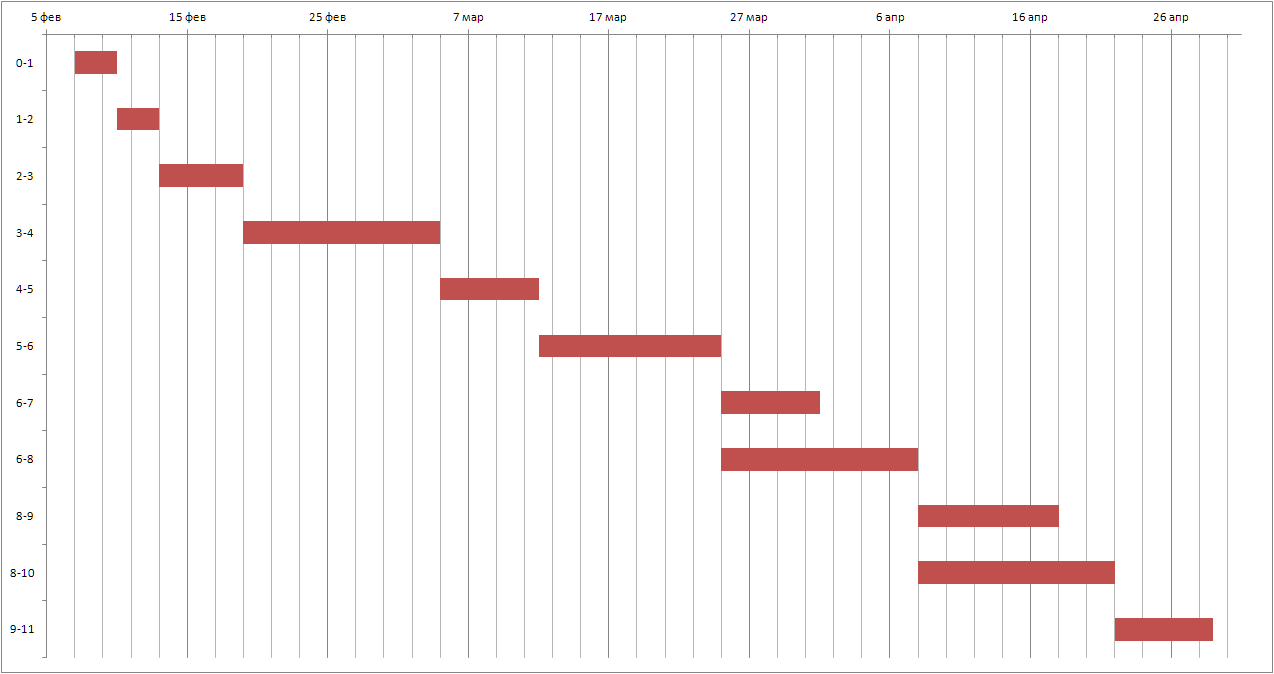
\includegraphics [scale=0.5] {gantt}
  \caption{Диаграмма Ганта проводимых работ} 
  \label{img:gant_diagram}  
\end{figure}

\begin{center}
 \renewcommand\multirowsetup{\centering}
 \begin{longtable}[h]{| >{\centering}m{2cm} | >{\centering}m{4cm} | >{\centering}m{4cm} | >{\centering}m{5cm}|}
	\captionsetup{justification=raggedright}
	\caption{Занятость исполнителей} \label{table:workers_dates} \tabularnewline
	\hline

 \rowcolor{Gray}  Код работы  & Дата начала & Дата окончания &  Исполнитель \tabularnewline \hline \endfirsthead   \hline
 \multicolumn{4}{|c|}{\small\slshape (продолжение таблицы \ref{table:workers_dates})}        \tabularnewline \hline
 \rowcolor{Gray}  Код работы  & Дата начала & Дата окончания &  Исполнитель \tabularnewline \hline
                                              \endhead        \hline
 % \multicolumn{3}{|r|}{\small\slshape продолжение следует}  \tabularnewline \hline
                                              \endfoot        \hline
                                              \endlastfoot

0-1 & 07.02.2014 & 07.02.2014 & Ведущий программист \tabularnewline \hline
1-2 & 09.02.2014 & 12.02.2014 & Ведущий программист \tabularnewline \hline
2-3 & 13.02.2014 & 18.02.2014 & Ведущий программист \tabularnewline \hline
3-4 & 19.02.2014 & 04.03.2014 & Ведущий программист \tabularnewline \hline
4-5 & 05.03.2014 & 11.03.2014 & Ведущий программист \tabularnewline \hline
5-6 & 12.03.2014 & 24.03.2014 & Ведущий программист \tabularnewline \hline
6-7 & 25.03.2014 & 31.03.2014 & Программист \tabularnewline \hline
6-8 & 25.03.2014 & 07.04.2014 & Ведущий программист \tabularnewline \hline
8-9 & 08.04.2014 & 17.04.2014 & Программист \tabularnewline \hline
8-10 &08.04.2014 & 21.04.2014 & Ведущий программист \tabularnewline \hline
9-11 & 22.04.2014 & 28.04.2014 & Ведущий программист \tabularnewline \hline
\end{longtable}
\end{center}

\FloatBarrier